\section{Ablation Analysis / Visualizations}%
\label{sec:ablation}
\begin{figure}[t]
  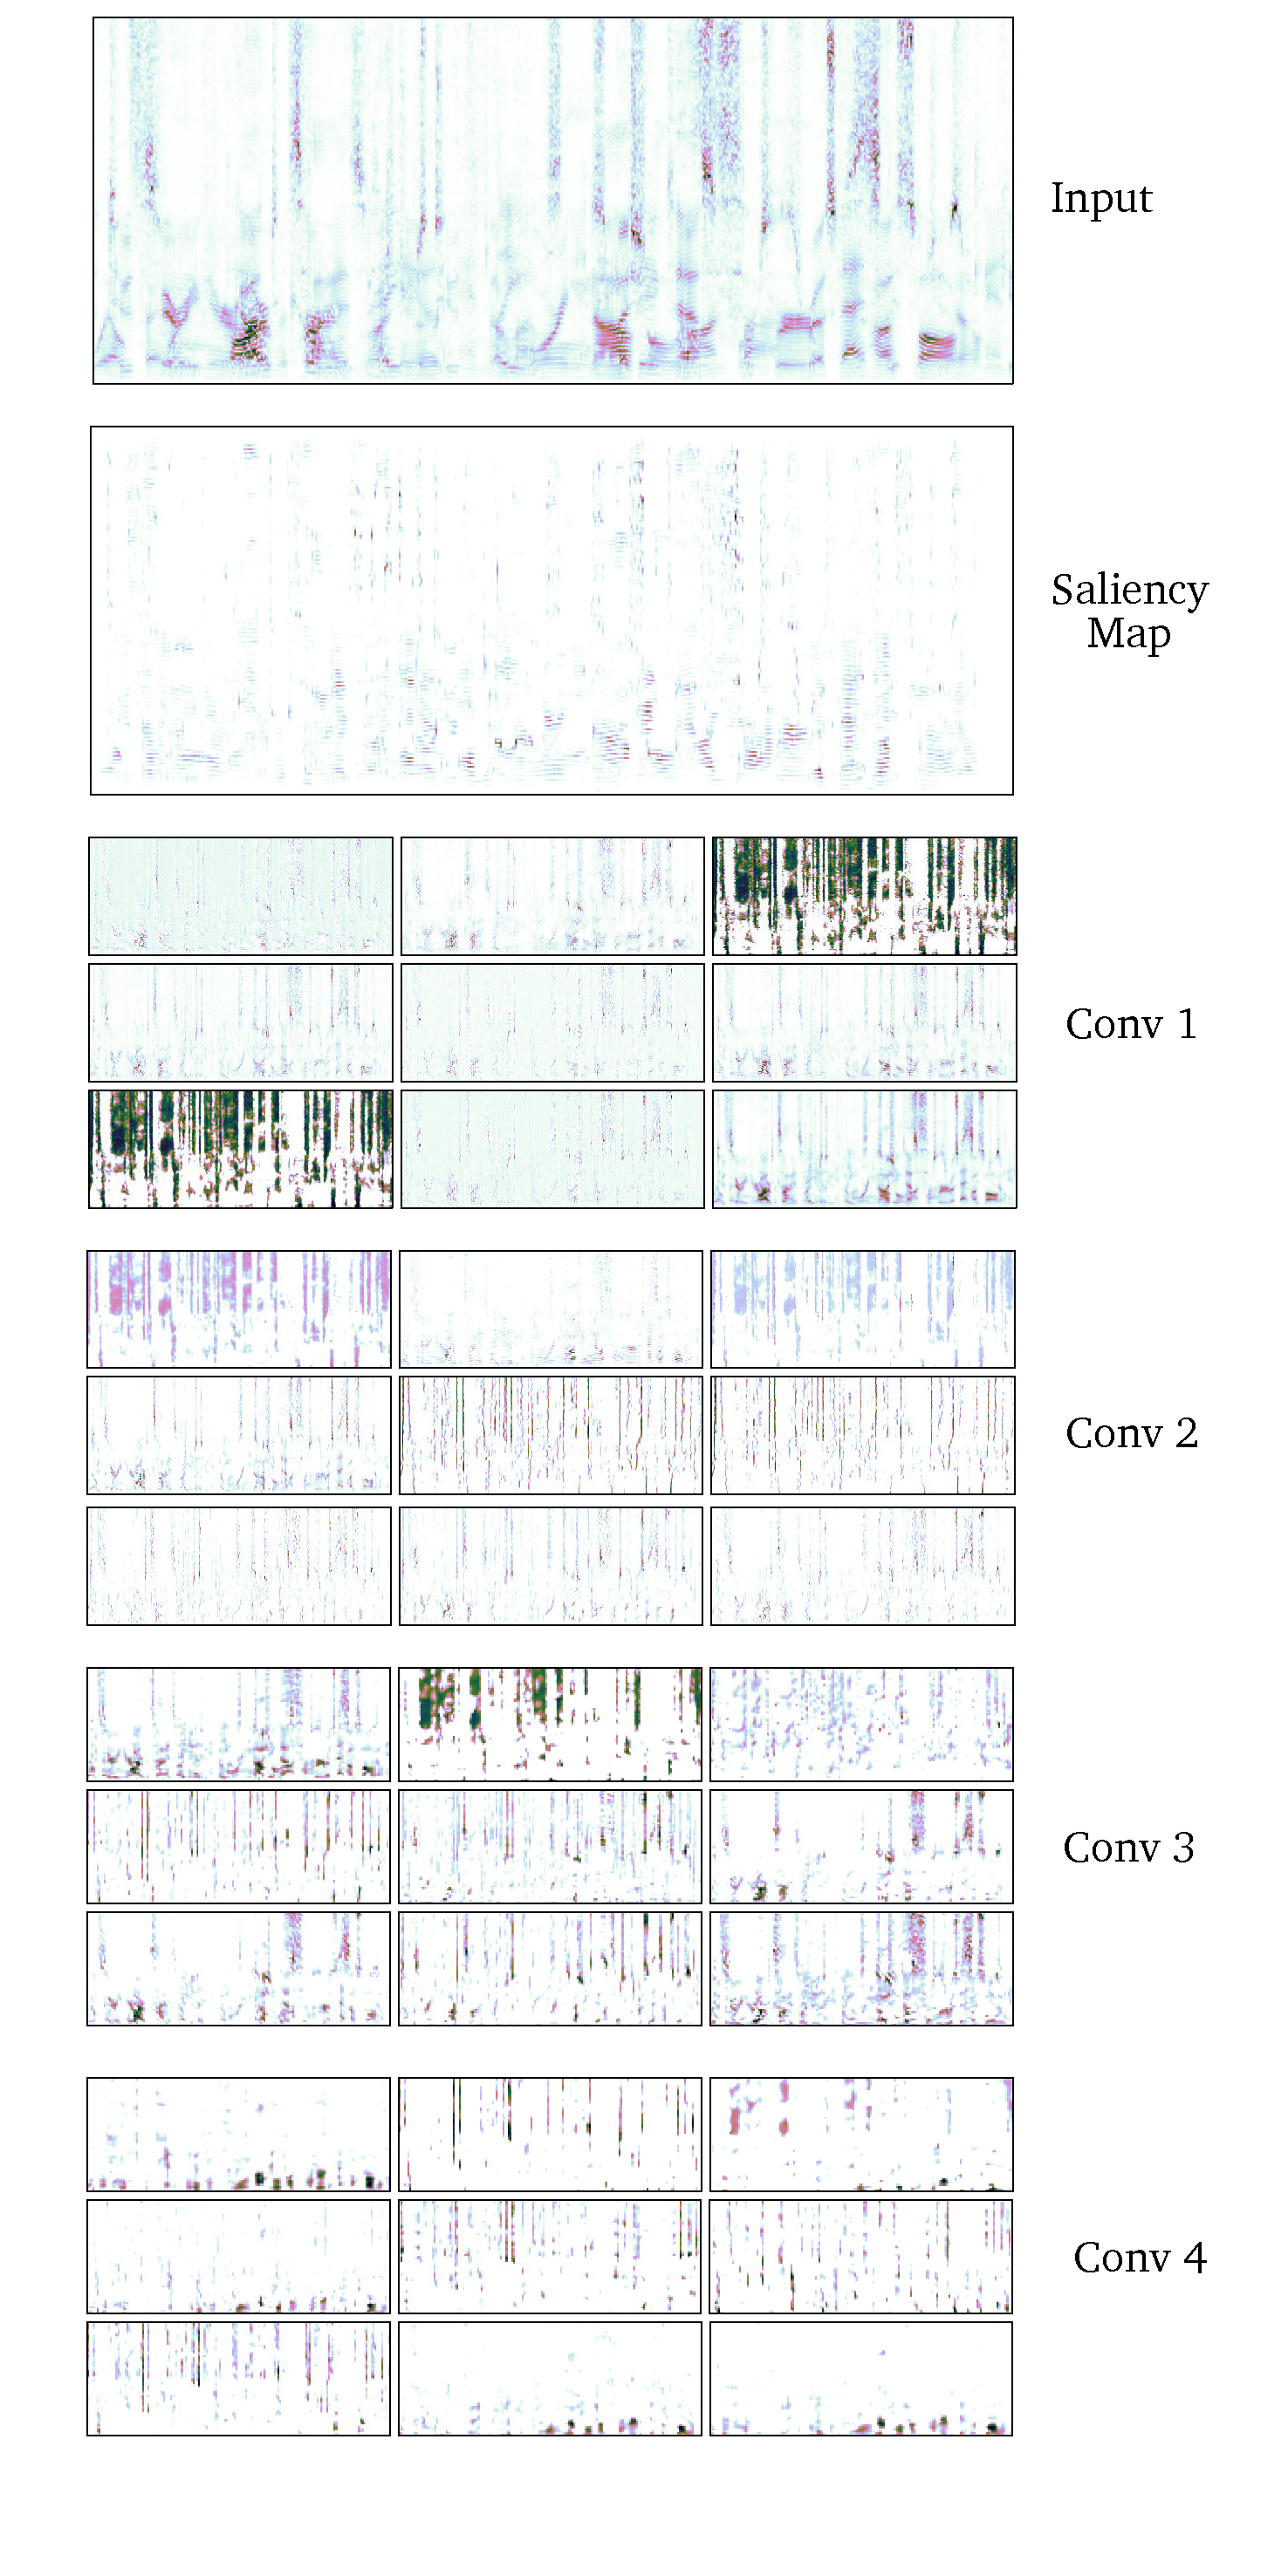
\includegraphics[width=\columnwidth, height=0.7\paperheight, keepaspectratio]{Chapters/08_Analysis_CountNet/dsc/figures/outputs.pdf}
  \caption{Illustration of intermediate outputs from the proposed CRNN for each convolutional layer for a given input with \(k=3\) speakers. Saliency map shows positive saliency of guided backpropagation~\cite{Springenberg14}. For each convolutional layer the nine most relevant filters were selected based on their loss with respect to the input.}%
\label{fig:convoutputs}
\end{figure}
% Select best performing system (CRNN, Classification, STFT) and analyse how it achieves the performance.
In the previous section we showed the effectiveness of the CRNN based model.
Even though \emph{CRNN} achieves very good performance under various conditions, it still remains unclear what strategy the model pursues.
To gain more insight, we conducted a visual analysis based on salience map representations~\cite{Simonyan13}.
% taken from https://github.com/Lasagne/Recipes/blob/master/examples/Saliency%20Maps%20and%20Guided%20Backpropagation.ipynb
In the deep learning context, saliency maps are visualizations that are able to show which specific input elements a neural network used for a particular prediction. This allows an object classifier to be used for object localization or in the case of audio spectrograms, which time frequency bins are most relevant.
The common idea is to compute the gradient of the model's prediction with respect to the input, holding the weights fixed. This determines which input elements need to be changed the least to affect the prediction the most.
\par
In this work we used guided backpropagations, first introduced in~\cite{Springenberg14} and successfully deployed in~\cite{schluter16} to compute a saliency map for singing voice detection.
For a given input spectrogram of a three speaker mixture, we depicted the saliency map in Figure~\ref{fig:convoutputs}.
The saliency map indicates that our proposed model does not rely much on the overlapped parts but instead utilize many of the single speaker time frequency bins.
Also, we can see that both, low frequency harmonic structures as well as many high frequency components such as plosives and fricative phonemes result in increased saliency.
For a more detailed analysis, we also visualized the filtered outputs of the successive convolutional layers.
While we cannot show all filter outputs (e.g. 64, for the first layer), instead for each filter, we compute its loss with respect to the input of the model using gradient update and sort the filters according to their loss.
Figure~\ref{fig:convoutputs} depicts the nine highest loss outputs per convolutional layer.
We can observe that while the first layer shows only low level variations of the input, already the second layer seems to be more abstract and emphasizes phoneme segmentations based on mid and high frequency content.
While filter outputs of layer 3 and 4 also show more low-frequency content such as the harmonic signals, the overall visual impression is that the proposed CRNN focuses on the temporal segmentation of phonemes.
\par
This leads to the hypothesis that the CRNN model learned the aggregated phoneme or syllable activity of all speakers in a fixed, given excerpt.
% \captionof{table}{Binary Logit Regression}\label{Binary Logit Regression}\begin{center}
% \begin{tabular}{lclc}
% \toprule
% \textbf{Dep. Variable:} &      error       & \textbf{  No. Observations:  } &     2000   \\
% \textbf{Model:}         &      Logit       & \textbf{  Df Residuals:      } &     1998   \\
% \textbf{Method:}        &       MLE        & \textbf{  Df Model:          } &        1   \\
% \textbf{Date:}          & Mon, 29 Jan 2018 & \textbf{  Pseudo R-squ.:     } &  0.01108   \\
% \textbf{Time:}          &     16:38:38     & \textbf{  Log-Likelihood:    } &   -1370.9  \\
% \textbf{converged:}     &       True       & \textbf{  LL-Null:           } &   -1386.3  \\
% \textbf{ }              &                  & \textbf{  LLR p-value:       } & 2.980e-08  \\
% \bottomrule
% \end{tabular}
% %\caption{Logit Regression Results}
% \end{center}
If that is the case, it would mean that the speaker count estimate would be affected if the speakers would speak slower or faster in relation to the fixed input window (speaking rate).
We therefore want to see if very slow or very fast speakers significantly increase the error of our proposed CRNN model.
In turn we define a null hypothesis that there is no association between the speaker count error probability and the value of the \emph{speaking rate}.
\par
To verify our hypothesis, we created another experiment based on the \emph{TIMIT} dataset.
It comes with phoneme and word level annotations, from which the speaking rate (defined as syllables per second) can be computed for each input sample~\cite{Jiao16}.
To reduce the influence of the different acoustical environment in TIMIT compared to Libri Speech, we retrained the CRNN classification model on the \emph{TIMIT} training dataset, using the same parameters as described in Section~\ref{sec:training}.
At test time we randomly generated 5 seconds excerpts of \(k=6\) from the TIMIT test subset and predicted the error \(E(k) = \hat{k} - k\) for each CRNN output.
We grouped the estimates into three classes: \(E(k) = 0\) (correct response), \(E(k) > 0\) (overestimation), \(E(k) < 0\) (underestimation).
For \(k=6\) we ended up with two groups of results because overestimation did not take place.
From the remaining two groups \emph{underestimation} and \emph{correct} responses we randomly selected 1000 samples each, resulting in an total sample size of \(n=2000\).
For these samples we computed an average speaking rate of \(3.40\) syllables per second and a standard deviation of \(0.2\).
We chose a Generalized Linear Model (GLM) for the statistical test, as described in~\cite{jaeger08}.
This allows us model the results with a binary logit regression model that turns the mean of E into a binomial distributed probability modeled by log linear values: \(\mbox{logit}(E) \sim \mbox{Intercept} + \beta \cdot{\mbox{Speaking Rate}}\).
\begin{table}[h]
\caption{Results of a binary logit regression test for the dependent variable \emph{correct response} over the independent variable \emph{speaking rate}. The results are based on $n=2000$ randomly drawn results of the CRNN model trained and evaluated on the TIMIT dataset.}%
\label{tab:logit}
\begin{center}
\begin{tabular}{lcccc}
\toprule
                        & \textbf{coef} & \textbf{std err} & \textbf{z} & \textbf{P$>$$|$z$|$} \\
\midrule
\textbf{speaking rate} &      -1.2697   &        0.232     &     -5.477  &         0.000        \\
\textbf{intercept}          &      4.3213  &        0.790     &    5.468  &         0.000  \\
\bottomrule
\end{tabular}
\end{center}
\end{table}
The results of our test are shown in Table~\ref{tab:logit} and indicate the speaking rate has statistically significant influence on the error \(p < 0.05, df=1, \textrm{Pseudo}\ R^2=0.0111\).
To better understand the effect of our predictor, we computed an odds ratio \(\exp(\mbox{speaking rate}) = 0.28\).
This indicates that a decrease in speaking rate of 1 syllable per second will increase the likeliness of an underestimation error by 28 percent.
Even though this is considered as a small effect size, it gives an interesting hint for the strategy taken of our proposed model and also suggests that for improved robustness, training would benefit from a large variety of speaking rates.
Furthermore, it still remains unclear the model would suffer from languages with a speaking rate which is naturally higher or lower than English or Chinese (see~\cite{Osser64}).
